\chapter{Chapter XLIV}

\begin{verse}
So! now 'tis ended, like an old wife's story.\\!
\attrib{Webster}
\end{verse}

\lettrine{W}{hen} the first moments of surprise were over, Wilfred
of Ivanhoe
demanded of the Grand Master, as judge of the field, if he had manfully
and rightfully done his duty in the combat? ``Manfully and rightfully
hath it been done,'' said the Grand Master. ``I pronounce the maiden
free and guiltless--The arms and the body of the deceased knight are at
the will of the victor.''

``I will not despoil him of his weapons,'' said the Knight of Ivanhoe,
``nor condemn his corpse to shame--he hath fought for Christendom--God's
arm, no human hand, hath this day struck him down. But let his obsequies
be private, as becomes those of a man who died in an unjust
quarrel.--And for the maiden--''

He was interrupted by a clattering of horses' feet, advancing in such
numbers, and so rapidly, as to shake the ground before them; and the
Black Knight galloped into the lists. He was followed by a numerous band
of men-at-arms, and several knights in complete armour.

``I am too late,'' he said, looking around him. ``I had doomed
Bois-Guilbert for mine own property.--Ivanhoe, was this well, to take on
thee such a venture, and thou scarce able to keep thy saddle?''

``Heaven, my Liege,'' answered Ivanhoe, ``hath taken this proud man for
its victim. He was not to be honoured in dying as your will had
designed.''

``Peace be with him,'' said Richard, looking steadfastly on the corpse,
``if it may be so--he was a gallant knight, and has died in his steel
harness full knightly. But we must waste no time--Bohun, do thine
office!''

A Knight stepped forward from the King's attendants, and, laying his
hand on the shoulder of Albert de Malvoisin, said, ``I arrest thee of
High Treason.''

The Grand Master had hitherto stood astonished at the appearance of so
many warriors.--He now spoke.

``Who dares to arrest a Knight of the Temple of Zion, within the girth
of his own Preceptory, and in the presence of the Grand Master? and by
whose authority is this bold outrage offered?''

``I make the arrest,'' replied the Knight--``I, Henry Bohun, Earl of
Essex, Lord High Constable of England.''

``And he arrests Malvoisin,'' said the King, raising his visor, ``by the
order of Richard Plantagenet, here present.--Conrade Mont-Fitchet, it is
well for thee thou art born no subject of mine.--But for thee,
Malvoisin, thou diest with thy brother Philip, ere the world be a week
older.''

``I will resist thy doom,'' said the Grand Master.

``Proud Templar,'' said the King, ``thou canst not--look up, and behold
the Royal Standard of England floats over thy towers instead of thy
Temple banner!--Be wise, Beaumanoir, and make no bootless
opposition--Thy hand is in the lion's mouth.''

``I will appeal to Rome against thee,'' said the Grand Master, ``for
usurpation on the immunities and privileges of our Order.''

``Be it so,'' said the King; ``but for thine own sake tax me not with
usurpation now. Dissolve thy Chapter, and depart with thy followers to
thy next Preceptory, (if thou canst find one), which has not been made
the scene of treasonable conspiracy against the King of England--Or, if
thou wilt, remain, to share our hospitality, and behold our justice.''

``To be a guest in the house where I should command?'' said the Templar;
``never!--Chaplains, raise the Psalm, `Quare fremuerunt
Gentes?'--Knights, squires, and followers of the Holy Temple, prepare to
follow the banner of `Beau-seant!'\,''

The Grand Master spoke with a dignity which confronted even that of
England's king himself, and inspired courage into his surprised and
dismayed followers. They gathered around him like the sheep around the
watch-dog, when they hear the baying of the wolf. But they evinced not
the timidity of the scared flock--there were dark brows of defiance, and
looks which menaced the hostility they dared not to proffer in words.
They drew together in a dark line of spears, from which the white cloaks
of the knights were visible among the dusky garments of their retainers,
like the lighter-coloured edges of a sable cloud. The multitude, who had
raised a clamorous shout of reprobation, paused and gazed in silence on
the formidable and experienced body to which they had unwarily bade
defiance, and shrunk back from their front.

The Earl of Essex, when he beheld them pause in their assembled force,
dashed the rowels into his charger's sides, and galloped backwards and
forwards to array his followers, in opposition to a band so formidable.
Richard alone, as if he loved the danger his presence had provoked, rode
slowly along the front of the Templars, calling aloud, ``What, sirs!
Among so many gallant knights, will none dare splinter a spear with
Richard?--Sirs of the Temple! your ladies are but sun-burned, if they
are not worth the shiver of a broken lance?''

``The Brethren of the Temple,'' said the Grand Master, riding forward in
advance of their body, ``fight not on such idle and profane quarrel--and
not with thee, Richard of England, shall a Templar cross lance in my
presence. The Pope and Princes of Europe shall judge our quarrel, and
whether a Christian prince has done well in bucklering the cause which
thou hast to-day adopted. If unassailed, we depart assailing no one. To
thine honour we refer the armour and household goods of the Order which
we leave behind us, and on thy conscience we lay the scandal and offence
thou hast this day given to Christendom.''

With these words, and without waiting a reply, the Grand Master gave the
signal of departure. Their trumpets sounded a wild march, of an Oriental
character, which formed the usual signal for the Templars to advance.
They changed their array from a line to a column of march, and moved off
as slowly as their horses could step, as if to show it was only the will
of their Grand Master, and no fear of the opposing and superior force,
which compelled them to withdraw.

``By the splendour of Our Lady's brow!'' said King Richard, ``it is pity
of their lives that these Templars are not so trusty as they are
disciplined and valiant.''

The multitude, like a timid cur which waits to bark till the object of
its challenge has turned his back, raised a feeble shout as the rear of
the squadron left the ground.

During the tumult which attended the retreat of the Templars, Rebecca
saw and heard nothing--she was locked in the arms of her aged father,
giddy, and almost senseless, with the rapid change of circumstances
around her. But one word from Isaac at length recalled her scattered
feelings.

``Let us go,'' he said, ``my dear daughter, my recovered treasure--let
us go to throw ourselves at the feet of the good youth.''

``Not so,'' said Rebecca, ``O no--no--no--I must not at this moment dare
to speak to him--Alas! I should say more than--No, my father, let us
instantly leave this evil place.''

``But, my daughter,'' said Isaac, ``to leave him who hath come forth
like a strong man with his spear and shield, holding his life as
nothing, so he might redeem thy captivity; and thou, too, the daughter
of a people strange unto him and his--this is service to be thankfully
acknowledged.''

``It is--it is--most thankfully--most devoutly acknowledged,'' said
Rebecca--``it shall be still more so--but not now--for the sake of thy
beloved Rachel, father, grant my request--not now!''

``Nay, but,'' said Isaac, insisting, ``they will deem us more thankless
than mere dogs!''

``But thou seest, my dear father, that King Richard is in presence, and
that---''

``True, my best--my wisest Rebecca!--Let us hence--let us hence!--Money
he will lack, for he has just returned from Palestine, and, as they say,
from prison--and pretext for exacting it, should he need any, may arise
out of my simple traffic with his brother John. Away, away, let us
hence!''

And hurrying his daughter in his turn, he conducted her from the lists,
and by means of conveyance which he had provided, transported her safely
to the house of the Rabbi Nathan.

The Jewess, whose fortunes had formed the principal interest of the day,
having now retired unobserved, the attention of the populace was
transferred to the Black Knight. They now filled the air with ``Long
life to Richard with the Lion's Heart, and down with the usurping
Templars!''

``Notwithstanding all this lip-loyalty,'' said Ivanhoe to the Earl of
Essex, ``it was well the King took the precaution to bring thee with
him, noble Earl, and so many of thy trusty followers.''

The Earl smiled and shook his head.

``Gallant Ivanhoe,'' said Essex, ``dost thou know our Master so well,
and yet suspect him of taking so wise a precaution! I was drawing
towards York having heard that Prince John was making head there, when I
met King Richard, like a true knight-errant, galloping hither to achieve
in his own person this adventure of the Templar and the Jewess, with his
own single arm. I accompanied him with my band, almost maugre his
consent.''

``And what news from York, brave Earl?'' said Ivanhoe; ``will the rebels
bide us there?''

``No more than December's snow will bide July's sun,'' said the Earl;
``they are dispersing; and who should come posting to bring us the news,
but John himself!''

``The traitor! the ungrateful insolent traitor!'' said Ivanhoe; ``did
not Richard order him into confinement?''

``O! he received him,'' answered the Earl, ``as if they had met after a
hunting party; and, pointing to me and our men-at-arms, said, `Thou
seest, brother, I have some angry men with me--thou wert best go to our
mother, carry her my duteous affection, and abide with her until men's
minds are pacified.'\,''

``And this was all he said?'' enquired Ivanhoe; ``would not any one say
that this Prince invites men to treason by his clemency?''

``Just,'' replied the Earl, ``as the man may be said to invite death,
who undertakes to fight a combat, having a dangerous wound unhealed.''

``I forgive thee the jest, Lord Earl,'' said Ivanhoe; ``but, remember, I
hazarded but my own life--Richard, the welfare of his kingdom.''

``Those,'' replied Essex, ``who are specially careless of their own
welfare, are seldom remarkably attentive to that of others--But let us
haste to the castle, for Richard meditates punishing some of the
subordinate members of the conspiracy, though he has pardoned their
principal.''

From the judicial investigations which followed on this occasion, and
which are given at length in the Wardour Manuscript, it appears that
Maurice de Bracy escaped beyond seas, and went into the service of
Philip of France; while Philip de Malvoisin, and his brother Albert, the
Preceptor of Templestowe, were executed, although Waldemar Fitzurse, the
soul of the conspiracy, escaped with banishment; and Prince John, for
whose behoof it was undertaken, was not even censured by his
good-natured brother. No one, however, pitied the fate of the two
Malvoisins, who only suffered the death which they had both well
deserved, by many acts of falsehood, cruelty, and oppression.

Briefly after the judicial combat, Cedric the Saxon was summoned to the
court of Richard, which, for the purpose of quieting the counties that
had been disturbed by the ambition of his brother, was then held at
York. Cedric tushed and pshawed more than once at the message--but he
refused not obedience. In fact, the return of Richard had quenched every
hope that he had entertained of restoring a Saxon dynasty in England;
for, whatever head the Saxons might have made in the event of a civil
war, it was plain that nothing could be done under the undisputed
dominion of Richard, popular as he was by his personal good qualities
and military fame, although his administration was wilfully careless,
now too indulgent, and now allied to despotism.

But, moreover, it could not escape even Cedric's reluctant observation,
that his project for an absolute union among the Saxons, by the marriage
of Rowena and Athelstane, was now completely at an end, by the mutual
dissent of both parties concerned. This was, indeed, an event which, in
his ardour for the Saxon cause, he could not have anticipated, and even
when the disinclination of both was broadly and plainly manifested, he
could scarce bring himself to believe that two Saxons of royal descent
should scruple, on personal grounds, at an alliance so necessary for the
public weal of the nation. But it was not the less certain: Rowena had
always expressed her repugnance to Athelstane, and now Athelstane was no
less plain and positive in proclaiming his resolution never to pursue
his addresses to the Lady Rowena. Even the natural obstinacy of Cedric
sunk beneath these obstacles, where he, remaining on the point of
junction, had the task of dragging a reluctant pair up to it, one with
each hand. He made, however, a last vigorous attack on Athelstane, and
he found that resuscitated sprout of Saxon royalty engaged, like country
squires of our own day, in a furious war with the clergy.

It seems that, after all his deadly menaces against the Abbot of Saint
Edmund's, Athelstane's spirit of revenge, what between the natural
indolent kindness of his own disposition, what through the prayers of
his mother Edith, attached, like most ladies, (of the period,) to the
clerical order, had terminated in his keeping the Abbot and his monks in
the dungeons of Coningsburgh for three days on a meagre diet. For this
atrocity the Abbot menaced him with excommunication, and made out a
dreadful list of complaints in the bowels and stomach, suffered by
himself and his monks, in consequence of the tyrannical and unjust
imprisonment they had sustained. With this controversy, and with the
means he had adopted to counteract this clerical persecution, Cedric
found the mind of his friend Athelstane so fully occupied, that it had
no room for another idea. And when Rowena's name was mentioned the noble
Athelstane prayed leave to quaff a full goblet to her health, and that
she might soon be the bride of his kinsman Wilfred. It was a desperate
case therefore. There was obviously no more to be made of Athelstane;
or, as Wamba expressed it, in a phrase which has descended from Saxon
times to ours, he was a cock that would not fight.

There remained betwixt Cedric and the determination which the lovers
desired to come to, only two obstacles--his own obstinacy, and his
dislike of the Norman dynasty. The former feeling gradually gave way
before the endearments of his ward, and the pride which he could not
help nourishing in the fame of his son. Besides, he was not insensible
to the honour of allying his own line to that of Alfred, when the
superior claims of the descendant of Edward the Confessor were abandoned
for ever. Cedric's aversion to the Norman race of kings was also much
undermined,--first, by consideration of the impossibility of ridding
England of the new dynasty, a feeling which goes far to create loyalty
in the subject to the king ``de facto''; and, secondly, by the personal
attention of King Richard, who delighted in the blunt humour of Cedric,
and, to use the language of the Wardour Manuscript, so dealt with the
noble Saxon, that, ere he had been a guest at court for seven days, he
had given his consent to the marriage of his ward Rowena and his son
Wilfred of Ivanhoe.

The nuptials of our hero, thus formally approved by his father, were
celebrated in the most august of temples, the noble Minster of York. The
King himself attended, and from the countenance which he afforded on
this and other occasions to the distressed and hitherto degraded Saxons,
gave them a safer and more certain prospect of attaining their just
rights, than they could reasonably hope from the precarious chance of a
civil war. The Church gave her full solemnities, graced with all the
splendour which she of Rome knows how to apply with such brilliant
effect.

Gurth, gallantly apparelled, attended as esquire upon his young master
whom he had served so faithfully, and the magnanimous Wamba, decorated
with a new cap and a most gorgeous set of silver bells. Sharers of
Wilfred's dangers and adversity, they remained, as they had a right to
expect, the partakers of his more prosperous career.

But besides this domestic retinue, these distinguished nuptials were
celebrated by the attendance of the high-born Normans, as well as
Saxons, joined with the universal jubilee of the lower orders, that
marked the marriage of two individuals as a pledge of the future peace
and harmony betwixt two races, which, since that period, have been so
completely mingled, that the distinction has become wholly invisible.
Cedric lived to see this union approximate towards its completion; for
as the two nations mixed in society and formed intermarriages with each
other, the Normans abated their scorn, and the Saxons were refined from
their rusticity. But it was not until the reign of Edward the Third that
the mixed language, now termed English, was spoken at the court of
London, and that the hostile distinction of Norman and Saxon seems
entirely to have disappeared.

It was upon the second morning after this happy bridal, that the Lady
Rowena was made acquainted by her handmaid Elgitha, that a damsel
desired admission to her presence, and solicited that their parley might
be without witness. Rowena wondered, hesitated, became curious, and
ended by commanding the damsel to be admitted, and her attendants to
withdraw.

She entered--a noble and commanding figure, the long white veil, in
which she was shrouded, overshadowing rather than concealing the
elegance and majesty of her shape. Her demeanour was that of respect,
unmingled by the least shade either of fear, or of a wish to propitiate
favour. Rowena was ever ready to acknowledge the claims, and attend to
the feelings, of others. She arose, and would have conducted her lovely
visitor to a seat; but the stranger looked at Elgitha, and again
intimated a wish to discourse with the Lady Rowena alone. Elgitha had no
sooner retired with unwilling steps, than, to the surprise of the Lady
of Ivanhoe, her fair visitant kneeled on one knee, pressed her hands to
her forehead, and bending her head to the ground, in spite of Rowena's
resistance, kissed the embroidered hem of her tunic.

\begin{figure}
    \centering
    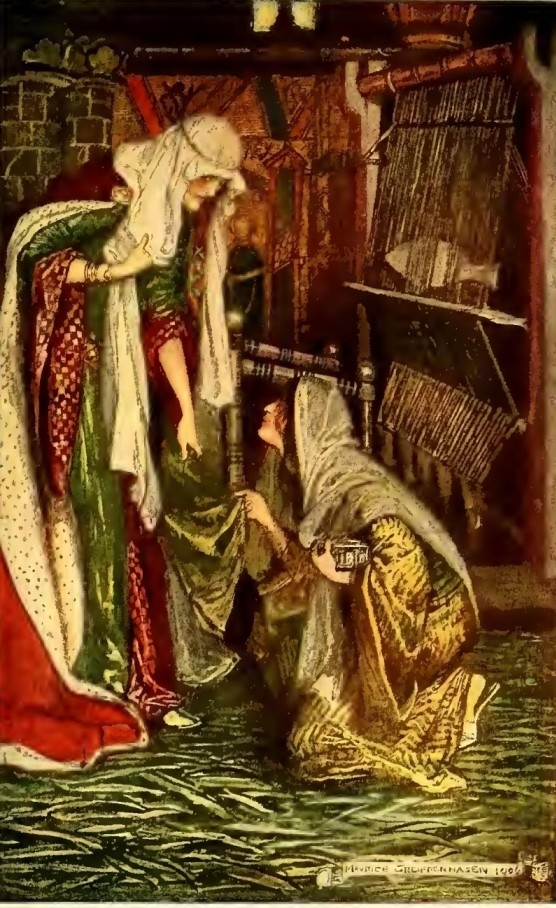
\includegraphics[height=.9\textheight]{ivanhoe/0597m}
    \caption{To the surprise of the Lady of Ivanhoe, her fair visitant
    kneeled on one knee.}
\end{figure}

``What means this, lady?'' said the surprised bride; ``or why do you
offer to me a deference so unusual?''

``Because to you, Lady of Ivanhoe,'' said Rebecca, rising up and
resuming the usual quiet dignity of her manner, ``I may lawfully, and
without rebuke, pay the debt of gratitude which I owe to Wilfred of
Ivanhoe. I am--forgive the boldness which has offered to you the homage
of my country--I am the unhappy Jewess, for whom your husband hazarded
his life against such fearful odds in the tiltyard of Templestowe.''

``Damsel,'' said Rowena, ``Wilfred of Ivanhoe on that day rendered back
but in slight measure your unceasing charity towards him in his wounds
and misfortunes. Speak, is there aught remains in which he or I can
serve thee?''

``Nothing,'' said Rebecca, calmly, ``unless you will transmit to him my
grateful farewell.''

``You leave England then?'' said Rowena, scarce recovering the surprise
of this extraordinary visit.

``I leave it, lady, ere this moon again changes. My father had a brother
high in favour with Mohammed Boabdil, King of Grenada--thither we go,
secure of peace and protection, for the payment of such ransom as the
Moslem exact from our people.''

``And are you not then as well protected in England?'' said Rowena. ``My
husband has favour with the King--the King himself is just and
generous.''

``Lady,'' said Rebecca, ``I doubt it not--but the people of England are
a fierce race, quarrelling ever with their neighbours or among
themselves, and ready to plunge the sword into the bowels of each other.
Such is no safe abode for the children of my people. Ephraim is an
heartless dove--Issachar an over-laboured drudge, which stoops between
two burdens. Not in a land of war and blood, surrounded by hostile
neighbours, and distracted by internal factions, can Israel hope to rest
during her wanderings.''

``But you, maiden,'' said Rowena--``you surely can have nothing to fear.
She who nursed the sick-bed of Ivanhoe,'' she continued, rising with
enthusiasm--``she can have nothing to fear in England, where Saxon and
Norman will contend who shall most do her honour.''

``Thy speech is fair, lady,'' said Rebecca, ``and thy purpose fairer;
but it may not be--there is a gulf betwixt us. Our breeding, our faith,
alike forbid either to pass over it. Farewell--yet, ere I go indulge me
one request. The bridal-veil hangs over thy face; deign to raise it, and
let me see the features of which fame speaks so highly.''

``They are scarce worthy of being looked upon,'' said Rowena; ``but,
expecting the same from my visitant, I remove the veil.''

She took it off accordingly; and, partly from the consciousness of
beauty, partly from bashfulness, she blushed so intensely, that cheek,
brow, neck, and bosom, were suffused with crimson. Rebecca blushed also,
but it was a momentary feeling; and, mastered by higher emotions, past
slowly from her features like the crimson cloud, which changes colour
when the sun sinks beneath the horizon.

``Lady,'' she said, ``the countenance you have deigned to show me will
long dwell in my remembrance. There reigns in it gentleness and
goodness; and if a tinge of the world's pride or vanities may mix with
an expression so lovely, how should we chide that which is of earth for
bearing some colour of its original? Long, long will I remember your
features, and bless God that I leave my noble deliverer united with--''

She stopped short--her eyes filled with tears. She hastily wiped them,
and answered to the anxious enquiries of Rowena--``I am well,
lady--well. But my heart swells when I think of Torquilstone and the
lists of Templestowe.--Farewell. One, the most trifling part of my duty,
remains undischarged. Accept this casket--startle not at its contents.''

Rowena opened the small silver-chased casket, and perceived a carcanet,
or neck lace, with ear-jewels, of diamonds, which were obviously of
immense value.

``It is impossible,'' she said, tendering back the casket. ``I dare not
accept a gift of such consequence.''

``Yet keep it, lady,'' returned Rebecca.--``You have power, rank,
command, influence; we have wealth, the source both of our strength and
weakness; the value of these toys, ten times multiplied, would not
influence half so much as your slightest wish. To you, therefore, the
gift is of little value,--and to me, what I part with is of much less.
Let me not think you deem so wretchedly ill of my nation as your commons
believe. Think ye that I prize these sparkling fragments of stone above
my liberty? or that my father values them in comparison to the honour of
his only child? Accept them, lady--to me they are valueless. I will
never wear jewels more.''

``You are then unhappy!'' said Rowena, struck with the manner in which
Rebecca uttered the last words. ``O, remain with us--the counsel of holy
men will wean you from your erring law, and I will be a sister to you.''

``No, lady,'' answered Rebecca, the same calm melancholy reigning in her
soft voice and beautiful features--``that--may not be. I may not change
the faith of my fathers like a garment unsuited to the climate in which
I seek to dwell, and unhappy, lady, I will not be. He, to whom I
dedicate my future life, will be my comforter, if I do His will.''

``Have you then convents, to one of which you mean to retire?'' asked
Rowena.

``No, lady,'' said the Jewess; ``but among our people, since the time of
Abraham downwards, have been women who have devoted their thoughts to
Heaven, and their actions to works of kindness to men, tending the sick,
feeding the hungry, and relieving the distressed. Among these will
Rebecca be numbered. Say this to thy lord, should he chance to enquire
after the fate of her whose life he saved.''

There was an involuntary tremour on Rebecca's voice, and a tenderness of
accent, which perhaps betrayed more than she would willingly have
expressed. She hastened to bid Rowena adieu.

``Farewell,'' she said. ``May He, who made both Jew and Christian,
shower down on you his choicest blessings! The bark that waits us hence
will be under weigh ere we can reach the port.''

She glided from the apartment, leaving Rowena surprised as if a vision
had passed before her. The fair Saxon related the singular conference to
her husband, on whose mind it made a deep impression. He lived long and
happily with Rowena, for they were attached to each other by the bonds
of early affection, and they loved each other the more, from the
recollection of the obstacles which had impeded their union. Yet it
would be enquiring too curiously to ask, whether the recollection of
Rebecca's beauty and magnanimity did not recur to his mind more
frequently than the fair descendant of Alfred might altogether have
approved.

Ivanhoe distinguished himself in the service of Richard, and was graced
with farther marks of the royal favour. He might have risen still
higher, but for the premature death of the heroic Coeur-de-Lion, before
the Castle of Chaluz, near Limoges. With the life of a generous, but
rash and romantic monarch, perished all the projects which his ambition
and his generosity had formed; to whom may be applied, with a slight
alteration, the lines composed by Johnson for Charles of Sweden--

\begin{verse}
His fate was destined to a foreign strand,\\
A petty fortress and an ``humble'' hand;\\
He left the name at which the world grew pale,\\
To point a moral, or adorn a \textsc{tale}.\\!
\end{verse}
